\documentclass{article}
\usepackage{venndiagram}
\usepackage{tikz}
\usetikzlibrary{patterns}

\begin{document}
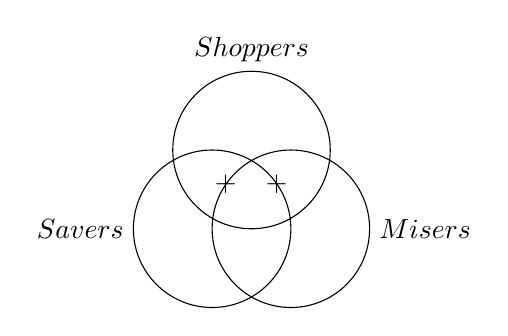
\begin{tikzpicture}[fill=gray]
    % %P1
    \draw (0.5,1) circle (1) (0.5,2) node [text=black,above] {$Shoppers$}
    (0,0) circle (1) (-1,0)  node [text=black,left] {$Savers$}
    (1,0) circle (1) (2,0)  node [text=black,right] {$Misers$}
    (0.82,.57) node [text=black, rotate=-45] {$\times $}
    (0.18,.57) node [text=black, rotate=-45] {$\times $};




    % P2
    % \scope
    % \clip (-2,-2) rectangle (2,2)
    % (0.5,1) circle (1)
    % (1,0) circle (1);
    % \fill[pattern=horizontal lines, pattern color=black] (1,0) circle (1);
    % \endscope

    % \scope
    % \clip (-2,-2) rectangle (2,2)
    % (0,0) circle (1)
    % (0.5,1) circle (1);
    % \fill[pattern=horizontal lines, pattern color=black] (0.5,1) circle (1);
    % \endscope

    % \draw (0.5,1) circle (1) (0.5,2) node [text=black,above] {$Liberals$}
    % (0,0) circle (1) (-1,0)  node [text=black,left] {$Greens$}
    % (1,0) circle (1) (2,0)  node [text=black,right] {$Conservatives$};














    % \draw (0.5,1) circle (1) (0.5,2) node [text=black,above] {$Performers$}
    % (0,0) circle (1) (-1,0)  node [text=black,left] {$Clowns$}
    % (1,0) circle (1) (2,0)  node [text=black,right] {$Artists$};

    % \fill[pattern=horizontal lines, pattern color=black] (0.5,1) circle (1);
    % \fill[color=white] (0,0) circle (1);
    % \fill[color=white] (1,0) circle (1);

    % \draw (0.5,1) circle (1) (0.5,2) node [text=black,above] {$Performers$}
    % (0,0) circle (1) (-1,0)  node [text=black,left] {$Clowns$}
    % (1,0) circle (1) (2,0)  node [text=black,right] {$Artists$}
    % (0.5,0.4) node [text=black] {$\times $};

    % \scope
    % \clip (-2,-2) rectangle (2,2)
    % (1,0) circle (1);
    % \fill[pattern=horizontal lines, pattern color=black] (0.5,1) circle (1);
    % \endscope

\end{tikzpicture}
\end{document}